\subsection{Persistenza dei dati}
Per il salvataggio persistente dei dati, abbiamo optato per un database in PostgresSQL.
Siamo partiti dal seguente schema per poi proseguire con una ristrutturazione:
\begin{figure}[H]
    \centering
    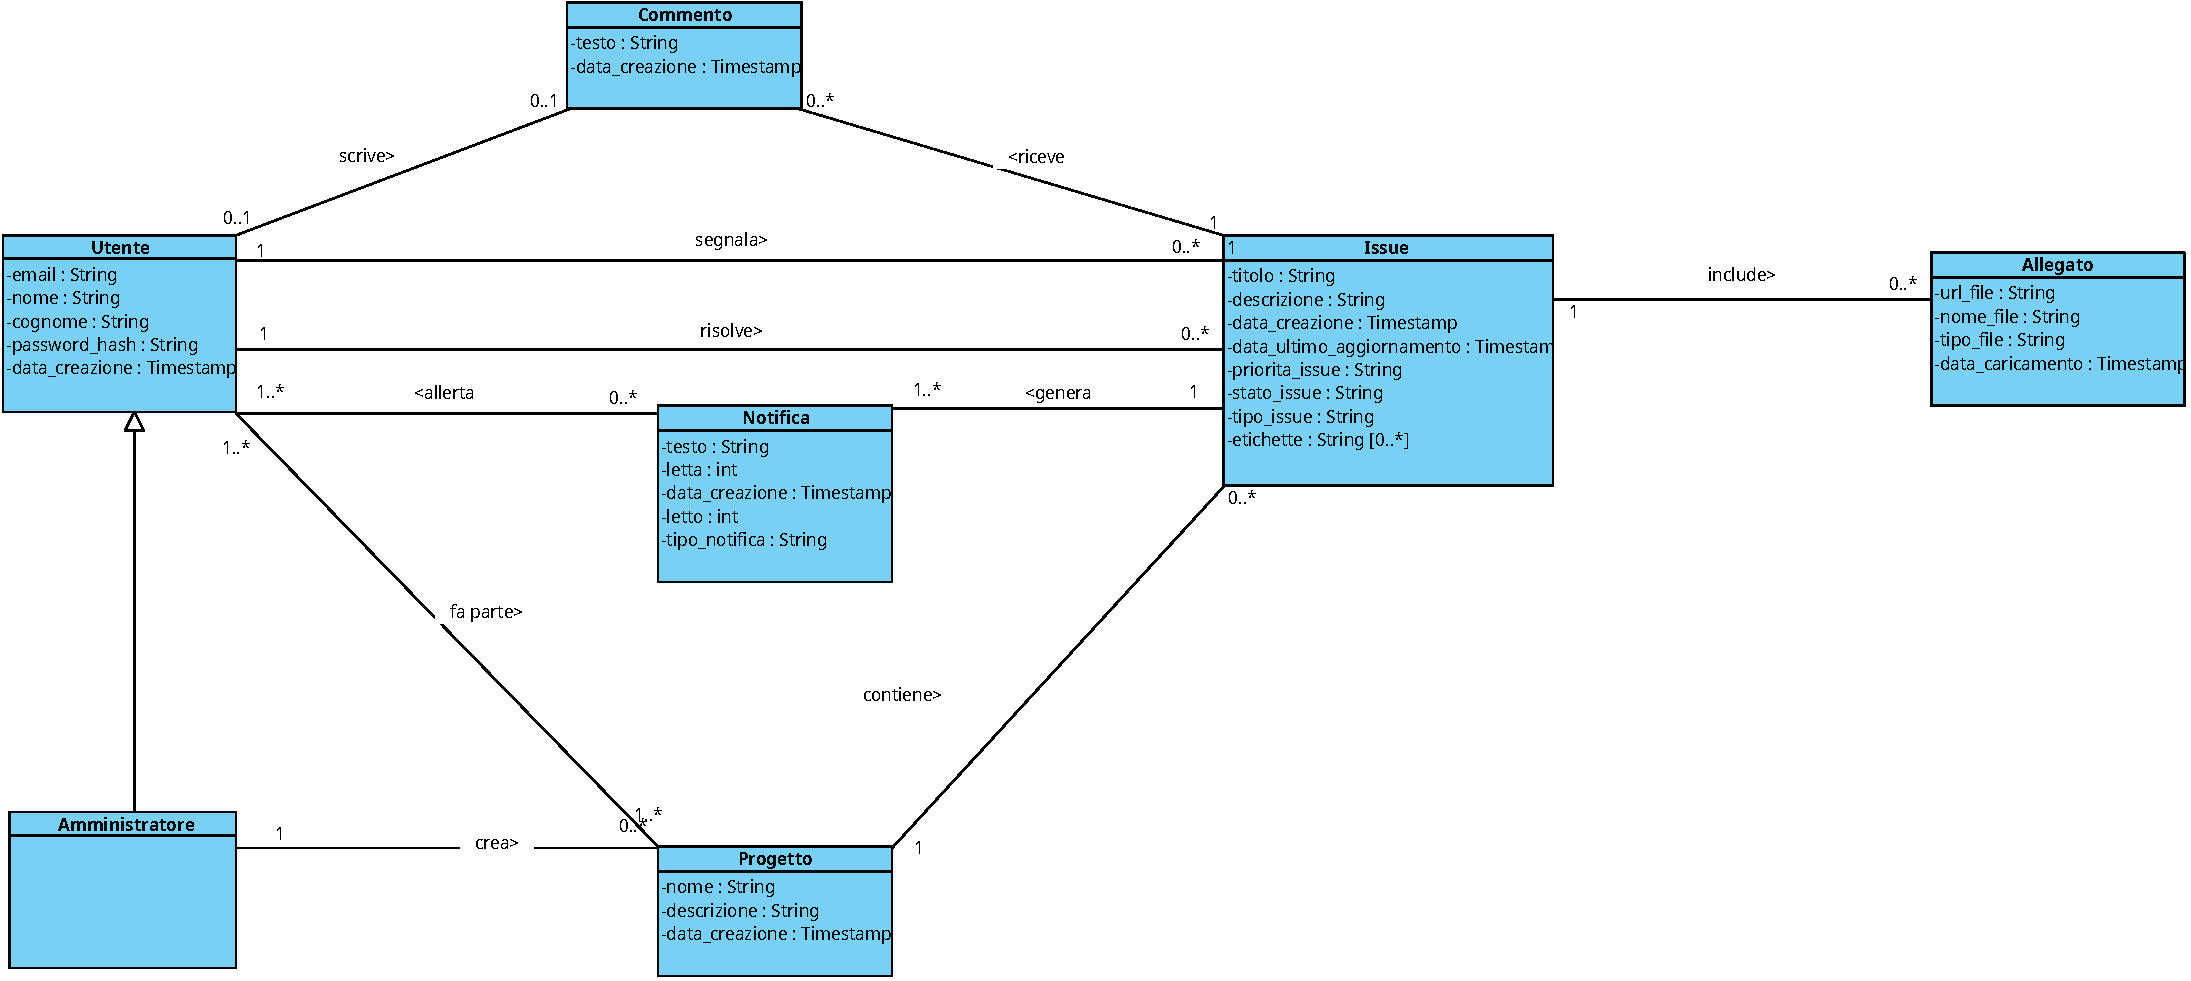
\includegraphics[width=1\textwidth]{DBVECCHIO.pdf}
    \caption{Schema UML}
\end{figure}
\newpage
\subsubsection{Ristrutturazione}
Abbiamo effettuato una ristrutturazione dello schema per migliorarne l'efficienza e prepararlo ad una traduzione in schema logico.
I passaggi effettuati sono stati i seguenti:
\begin{itemize}
    \item \textbf{Analisi delle ridondanze:} abbiamo individuato delle possibili ridondanze nelle associazioni tra utente, amministratore, issue e progetto. Abbiamo tuttavia deciso di mantenerle, data la necessità di effettuare operazioni come ad esempio vedere tutte le issue risolte da un utente, mantenendo queste operazioni semplici attraverso queste associazioni.
    \item \textbf{Eliminazione delle generalizzazioni:} Abbiamo rimosso l'unica generalizzazione presente: quella tra Utente ed Amministratore, accorpando tutto in Utente aggiungendo il campo "ruolo".
    \item \textbf{Eliminazione attributi multivalore:} Abbiamo rimosso l'unico attributo multivalore presente: etichette all'interno di Issue. Abbiamo creato l'entità Etichetta in modo da avere una visione e gestione più chiara delle etichette.
    \item \textbf{Eliminazione attributi strutturati:} Non erano presenti attributi strutturati.
    \item \textbf{Partizionamento/Accorpamento di entità e associazioni:} Non c'è stata necessità di accorpare nulla.
    \item \textbf{Scelta degli identificatori primari:} Per utente abbiamo scelto "email", per tutte le altre entità abbiamo inserito un campo "id".
\end{itemize}
\newpage
L'UML ristrutturato, alla fine, si presenta così:
\begin{figure}[H]
    \centering
    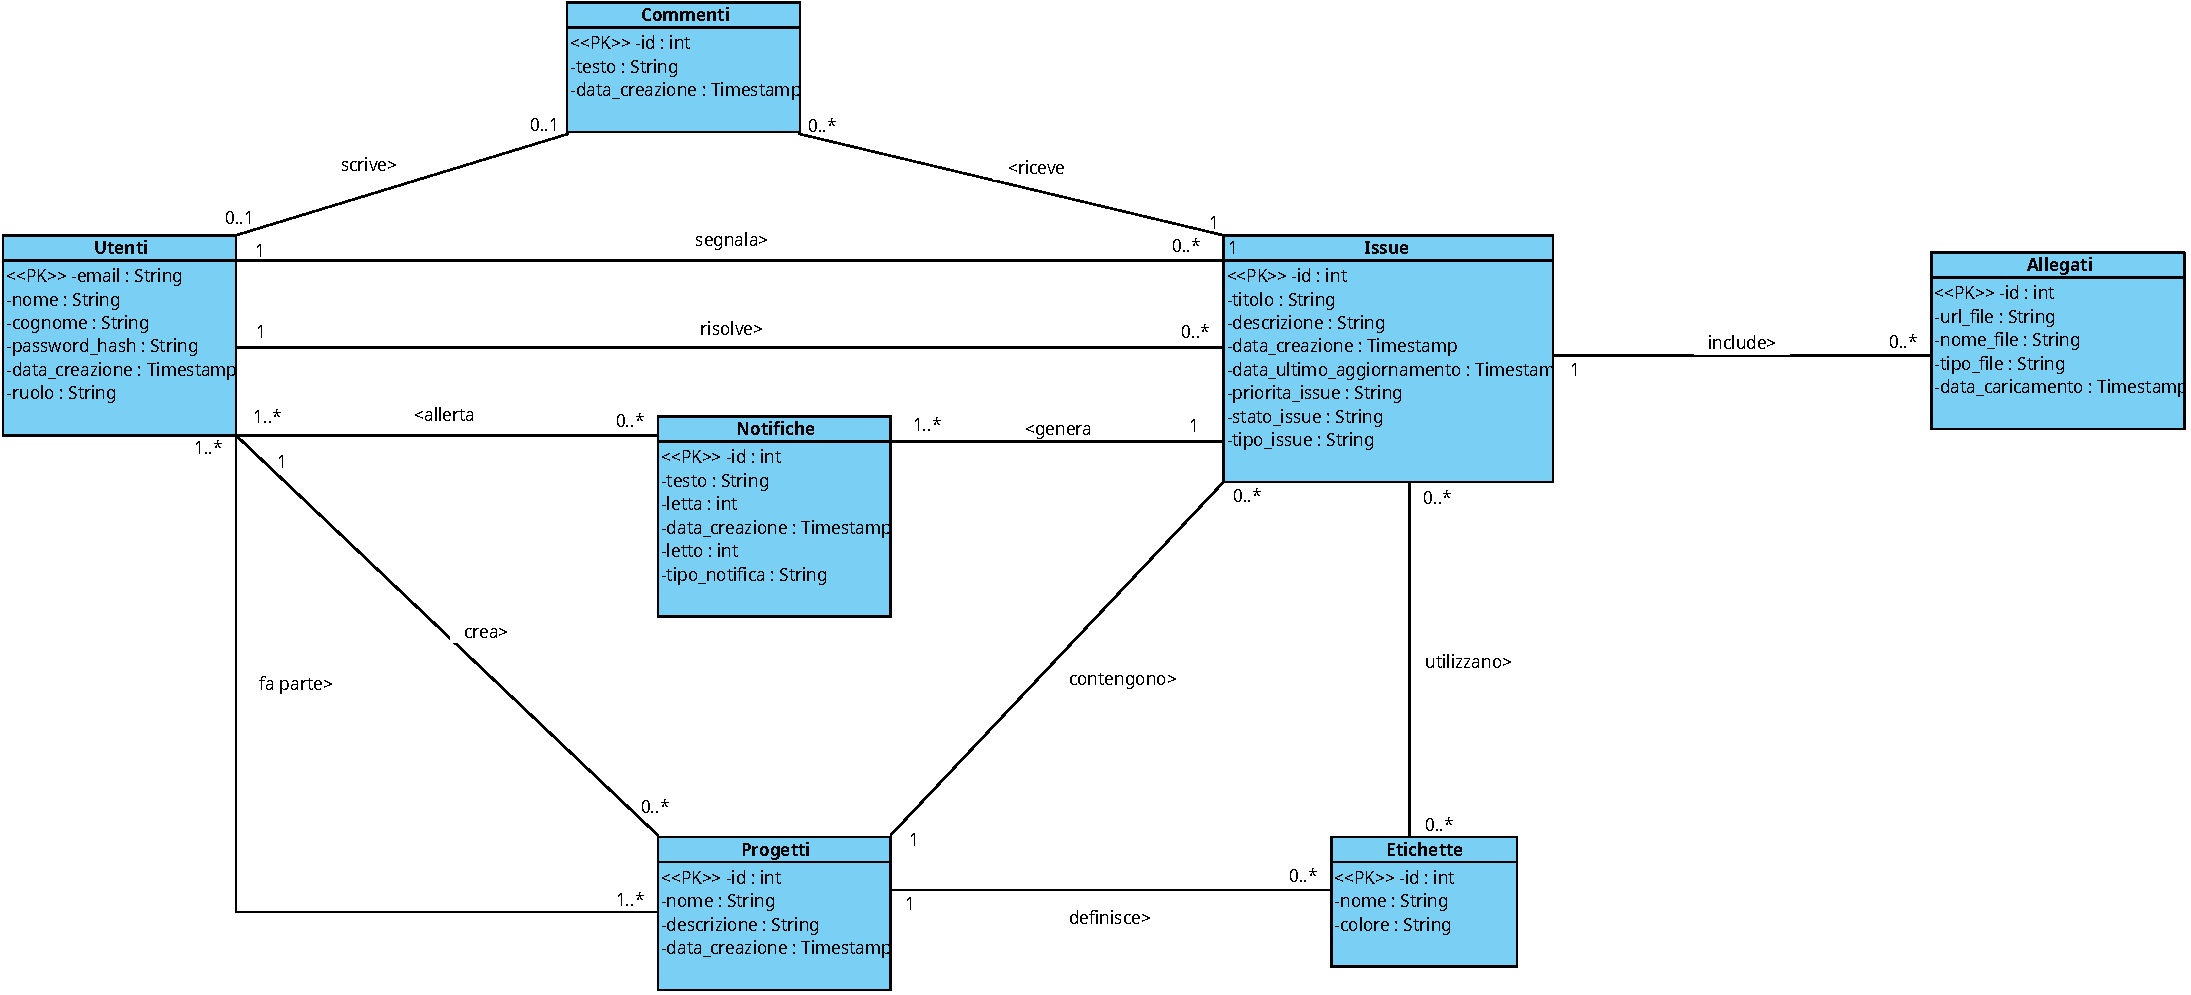
\includegraphics[width=1\textwidth]{DB.pdf}
    \caption{Schema UML ristrutturato}
\end{figure}
\subsubsection{Schema logico}
Lo schema logico derivato dalla ristrutturazione è il seguente:
\begin{itemize}
    \item \textbf{Utente}(\underline{email}, nome, cognome, password\_hash, data\_creazione, ruolo)

    \item \textbf{Progetto}(\underline{id}, nome, descrizione, \underline{\underline{id\_creatore}}, data\_creazione)\\
    \textit{id\_creatore} $\rightarrow$ Utente.email

    \item \textbf{ProgettoMembri}(\underline{\underline{\underline{id\_progetto}}}, \underline{\underline{\underline{email\_utente}}})\\
    \textit{id\_progetto} $\rightarrow$ Progetto.id\\
    \textit{email\_utente} $\rightarrow$ Utente.email

    \item \textbf{Issue}(\underline{id}, \underline{\underline{id\_progetto}}, \underline{\underline{email\_autore}}, \underline{\underline{email\_assegnatario}}, titolo, descrizione, data\_creazione, data\_ultimo\_aggiornamento, priorita\_issue, stato\_issue, tipo\_issue)\\
    \textit{id\_progetto} $\rightarrow$ Progetto.id\\
    \textit{email\_autore} $\rightarrow$ Utente.email\\
    \textit{email\_assegnatario} $\rightarrow$ Utente.email

    \item \textbf{Etichetta}(\underline{id}, \underline{\underline{id\_progetto}}, nome, colore)\\
    \textit{id\_progetto} $\rightarrow$ Progetto.id

    \item \textbf{IssueEtichette}(\underline{\underline{\underline{id\_issue}}}, \underline{\underline{\underline{id\_etichetta}}})\\
    \textit{id\_issue} $\rightarrow$ Issue.id\\
    \textit{id\_etichetta} $\rightarrow$ Etichetta.id

    \item \textbf{Commento}(\underline{id}, \underline{\underline{id\_issue}}, \underline{\underline{email\_autore}}, testo, data\_creazione)\\
    \textit{id\_issue} $\rightarrow$ Issue.id\\
    \textit{email\_autore} $\rightarrow$ Utente.email

    \item \textbf{Allegato}(\underline{id}, \underline{\underline{id\_issue}}, url\_file, nome\_file, tipo\_file, data\_caricamento)\\
    \textit{id\_issue} $\rightarrow$ Issue.id

    \item \textbf{Notifica}(\underline{id}, \underline{\underline{email\_utente}}, \underline{\underline{id\_issue}}, testo, letta, data\_creazione, tipo\_notifica)\\
    \textit{email\_utente} $\rightarrow$ Utente.email\\
    \textit{id\_issue} $\rightarrow$ Issue.id
\end{itemize}

\subsubsection{Funzioni, Trigger \& Varie}

\paragraph{Funzioni}
\begin{itemize}
    \item \textbf{aggiorna\_timestamp\_modifica():} funzione PL/pgSQL che aggiorna automaticamente il campo \texttt{data\_ultimo\_aggiornamento} al timestamp corrente ogni volta che una riga viene modificata.
\end{itemize}

\paragraph{Trigger}
\begin{itemize}
    \item \textbf{trg\_issue\_before\_update:} trigger attivato \texttt{BEFORE UPDATE} sulla tabella \texttt{Issue}. Per ogni riga aggiornata, invoca la funzione \texttt{aggiorna\_timestamp\_modifica()}, garantendo che il campo \texttt{data\_ultimo\_aggiornamento} rifletta sempre l'ultima modifica effettuata.
\end{itemize}

\paragraph{Tipi enumerativi (ENUM)}
Sono stati definiti i seguenti tipi enumerativi per vincolare i valori ammessi in determinati campi:
\begin{itemize}
    \item \textbf{priorita\_issue:} ALTA, BASSA, CRITICA, MEDIA, NESSUNA
    \item \textbf{stato\_issue:} ARCHIVIATA, CHIUSA, IN\_LAVORAZIONE, IN\_REVISIONE, RISOLTA, TODO
    \item \textbf{tipo\_issue:} BUG, DOCUMENTATION, FEATURE, QUESTION
    \item \textbf{tipo\_notifica:} ASSEGNATA, COMMENTO, CRITICA, MENZIONE, PROGETTO, RISOLTA
    \item \textbf{tipo\_ruolo:} AMMINISTRATORE, UTENTE
\end{itemize}

\paragraph{Indici}
Per migliorare le prestazioni delle query più frequenti, sono stati creati i seguenti indici:
\begin{itemize}
    \item \textbf{idx\_utenti\_email} su \texttt{Utente(email)}
    \item \textbf{idx\_progetti\_nome} su \texttt{Progetto(nome)}
    \item \textbf{idx\_progetto\_membri\_utente} su \texttt{ProgettoMembri(email\_utente)}
    \item \textbf{idx\_issue\_progetto} su \texttt{Issue(id\_progetto)}
    \item \textbf{idx\_issue\_assegnatario} su \texttt{Issue(email\_assegnatario)}
    \item \textbf{idx\_commenti\_issue} su \texttt{Commento(id\_issue)}
    \item \textbf{idx\_allegati\_issue} su \texttt{Allegato(id\_issue)}
    \item \textbf{idx\_notifiche\_utente} su \texttt{Notifica(email\_utente)}
    \item \textbf{idx\_notifiche\_letta} su \texttt{Notifica(email\_utente, letta)}
\end{itemize}

